%!TEX root = ../thesis.tex

\chapter{Spectroscopic reduction} % Main chapter title
\label{cha:reduction}

The work of this thesis relies on the use of \nir{} spectra obtained by the {CRIRES} instrument. Specifically 17 observations around 2.11-2.16\um{} which are detailed in \cref{tab:observations}.
This chapter contains an overview of the steps undertaken to extract astronomical spectra, focusing on the {CRIRES} instrument specifically.
A comparison between two different reduction pipelines for {CRIRES} is performed with the chosen pipeline used.
Details of the issues encountered with the reduction output are presented.
This chapter also includes the post reduction steps performed, specifically wavelength calibration and telluric correction.
The reduced spectra produced in this chapter will be analysed in \cref{cha:direct_recovery} and \cref{cha:model_comparison}.


\subsection{\nir{} reduction concepts}
\label{subsec:nirreduction}
In reducing \nir{} spectra, or any spectra in general a number of calibration steps that are performed to achieve the best possible e output such as removing signals arising from the detector. The main calibration steps required for \nir{} spectra are given below with examples from {CRIRES}. More information about the different effects with regards to CRIRES can be found in the CRIRES user manual and reduction cookbook.
%\begin{figure}[h]
%\centering
%%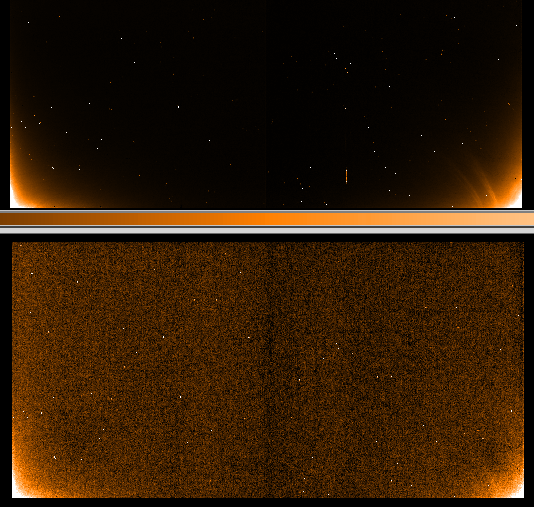
\includegraphics[width=0.4\textwidth]{figures/reduction/Master_Darks.png}
%\includegraphics[width=0.9\textwidth]{figures/reduction/master_darks_1.pdf}
%\caption[]{Master dark frames for exposure times of 3 and 180 seconds.
%Each master is created by averaging 3 images in which the detector received no incident light.
%Both frames are on the same scale and show dark current grows with exposure time.
%The colour has been inverted so that black is the recorded measurement.}
%\label{fig:darkcurrent}
%\end{figure}
\begin{figure}[h]
    \centering
    %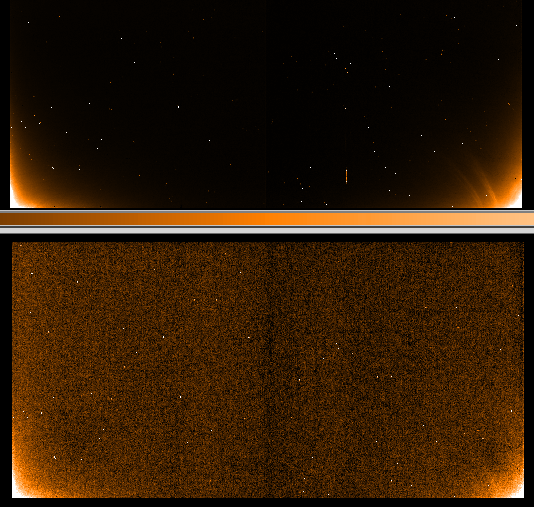
\includegraphics[width=0.4\textwidth]{figures/reduction/Master_Darks.png}
    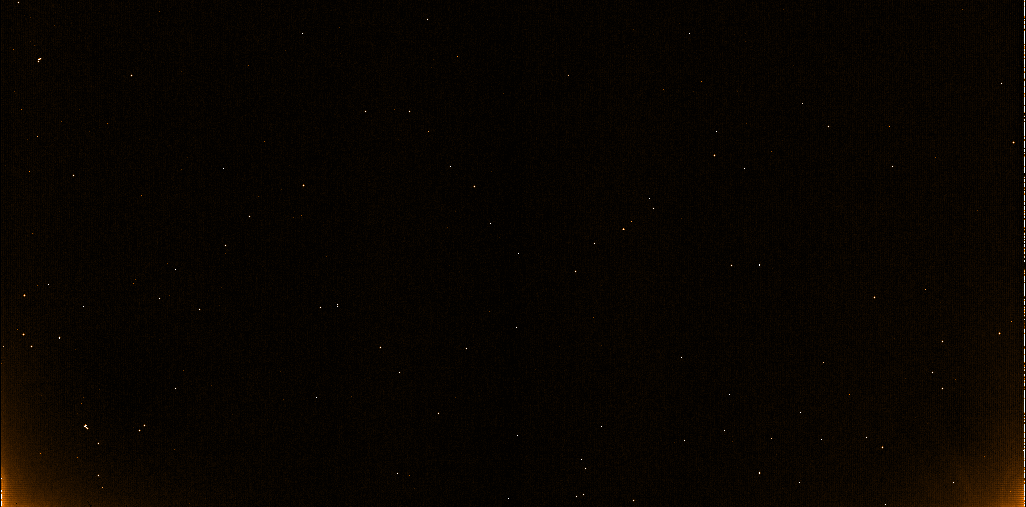
\includegraphics[width=0.45\textwidth]{figures/reduction/MasterDarkFlat_1.png}
    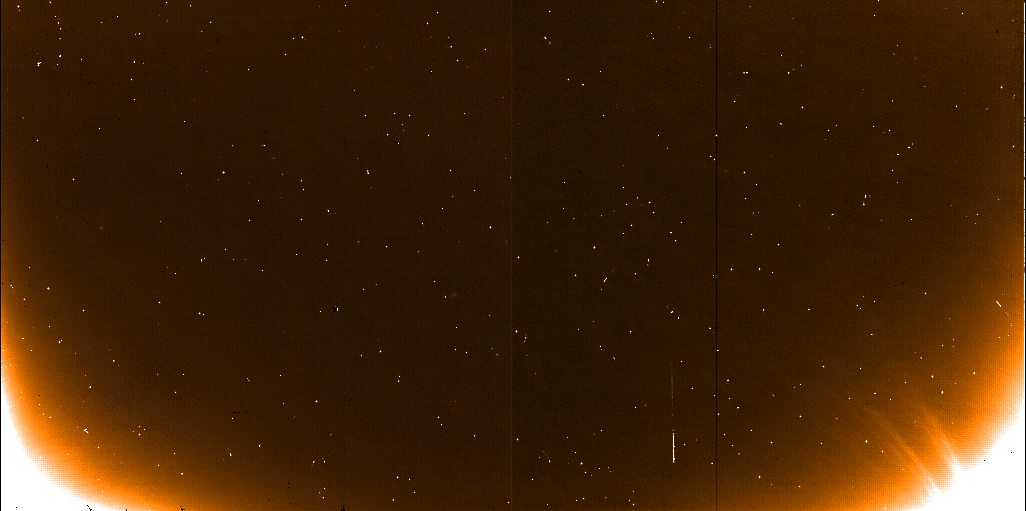
\includegraphics[width=0.45\textwidth]{figures/reduction/MasterDarkSpec_1.png}
    \caption[Example dark frames for different exposure times.]{Master dark frames for exposure times of 3 and 180 seconds.
Each master is created by averaging 3 images in which the detector received no incident light.
Both frames are on the same scale and show dark current grows with exposure time.
The colour has been inverted so that black is the recorded measurement.}
    \label{fig:darkcurrent_colour}
\end{figure}

\subsubsection{Dark Current}
\label{subsubsec:darkcurrent}
The dark current is a form of instrumental noise, in which the detector measures photons while not being illuminated.
It is the detection of thermal electrons moving inside the detector, creating spurious photon counts.
Calibration and removal of the dark current is performed by taking exposures in which the detector is not illuminated.
The detectors in the {CRIRES} instrument are cryogenically cooled to a temperature of \(\sim27\)\K{} (within 0.1\K{}) to significantly reduce the dark current, and to maintain consistency.
The electrical components of the {CRIRES} detectors create thermal energy while operational which impacts the dark current.
A strong ``glow'' is observed in the bottom corners of the {CRIRES} detector in \cref{fig:darkcurrent_colour} due to nearby amplifiers.
As per the {CRIRES} calibration plan, ``dark frames'' need to be taken for each exposure time used.
\Cref{fig:darkcurrent_colour} shows the master dark frame created from averaging three dark frames for exposure times of 3 seconds (for the flats) and 180 seconds (for the science), both on the same amplitude scale.
For the {CRIRES} detectors the dark current per pixel is around 0.2--0.4\,(\(e^{-}\)\si{\per\second}), while the glow at the two corners of the 180 second exposure shown here is \(\sim9000 / 180\approx50\)\,\(e^{-}\)\si{\per\second}.

%
%\begin{figure}[h]
%    \centering
%    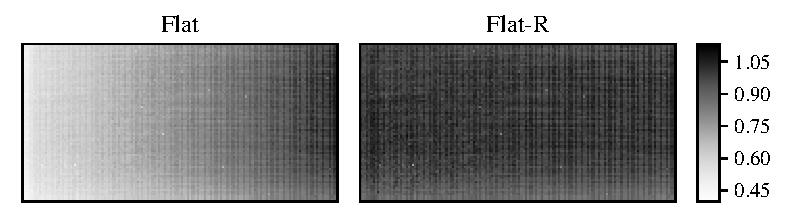
\includegraphics[width=0.9\textwidth]{figures/reduction/master_flats_1.pdf}
%    \caption[]{A flat-field image for detector \#1 before (left) and after (right) the non-linearity corrections are performed.
%    A perfect detector would have all pixels in the flat-field equal to 1.
%    \bf{\red{} Remove flat and flatR titles.}}
%    \label{fig:masterflats}
%\end{figure}


\begin{figure}[h]
    \centering
  %  \begin{tabular}[ll]
        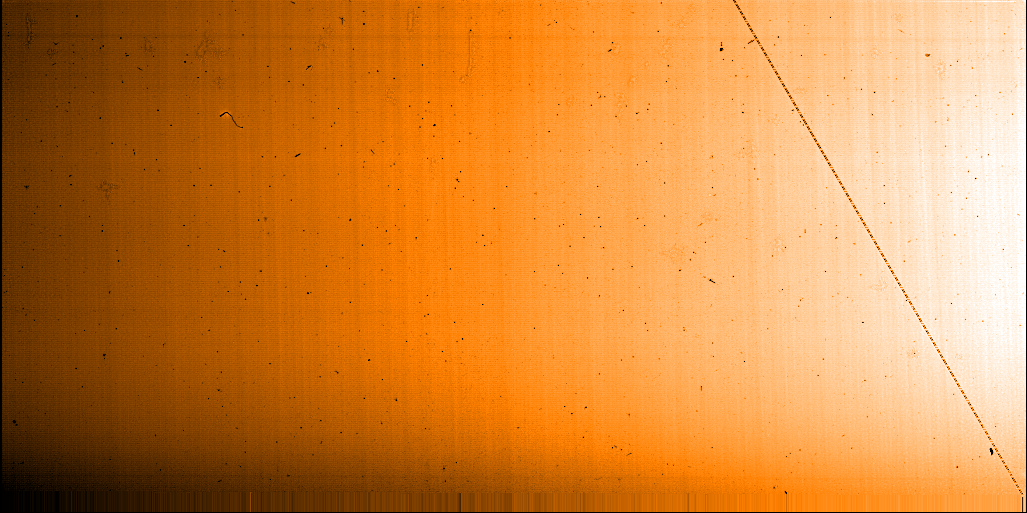
\includegraphics[width=0.45\textwidth]{figures/reduction/Flat_2.png} %
        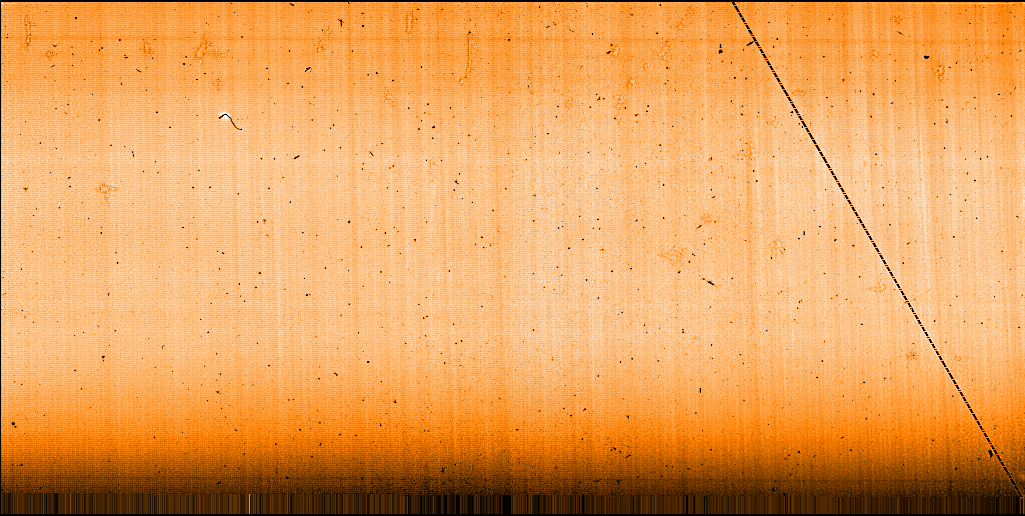
\includegraphics[width=0.45\textwidth]{figures/reduction/FlatR_2.png} %\\
    %\end{tabular}
    \caption[Example of flat-field correction.]{A flat-field image for detector \#2 before (left) and after (right) the non-linearity corrections are performed.}
    \label{fig:masterflats_colour}
\end{figure}


\subsubsection{Flat-field}
\label{subsubsec:flat-field}
No detector is truly perfect, with all pixels performing equally well.
To correct for pixel-to-pixel variations in photon sensitivity across the detector and for any distortions in the optical path, a flat-field correction is needed.
Exposures of a uniform\footnote{Ideally uniform intensity and spectral distribution} light source are taken, allowing the individual pixel-to-pixel sensitivity to be measured and corrected.
The flat-field frames are corrected for dark current by subtraction of the master dark frame with the appropriate exposure time.

The {CRIRES} detector suffers from non-linearities in sensitivity across the detector.
This can be seen in the flat-field image on the left of \cref{fig:masterflats_colour} where there is an intensity gradient from dark to light across the detector.
A set of coefficients for each pixel is provided by {ESO}\footnote{Available at \href{https://www.eso.org/sci/facilities/paranal/instruments/crires/tools.html}{https://www.eso.org/sci/facilities/paranal/instruments/crires/tools.html}} to apply the correction for the non-linearity of the detectors.
This also corrects for a slight difference in sensitivity between the pixels from the odd and even columns in the {CRIRES} detectors, commonly called the ``odd-even effect''.
The frame on the right of \cref{fig:masterflats_colour} has been corrected for the non-linearities.

The flat-field can also reveal defects in the detector e.g.\ dead pixels, dust and scratches: a large scratch is clearly visible in \cref{fig:masterflats_colour}.

\subsubsection{Nodding and Jitter}
\label{subsec:nod-jitter}
The technique of \emph{nodding} is used to remove sky emission, detector dark current, and glow.
First, an observation is divided into multiple separate exposures.
Between each exposure the telescope is moved to change the vertical position of the target in the slit.
The light from the star travels through a slightly different optical path and is recorded on a different part of the detector.
The frames from the two nod positions (A, B) are then subtracted (A - B) to remove the background measurement from each spectra.

A visual example of the nodding is shown in \cref{fig:nodimages}.
On the left are slices of 150 pixel columns from successive nod positions A and B as well as the difference A minus B.
On the right is a single pixel column from each image on the left.
The background signal at the level of 20--30 counts in the image is almost cancelled out by the opposite nod.
This efficiently removes the background signal/noise from the observed spectra target.

Observations of faint targets, that need long exposure times to achieve a sufficient \snr{}, are also broken up into multiple images so that the instrument glow from \cref{fig:darkcurrent_colour} does not saturate the detector.
A small random vertical offset is applied to each observation which ensures that all spectra at the same nod position do not consistently land on the same pixels each time.
This is known as the \emph{jitter} and allows for the correction of bad pixels and decreases the effect from any systematics of the detector.
As an example, the {CRIRES} observations analysed for the work performed in \cref{cha:direct_recovery,cha:model_comparison} were performed with an {ABBAABBA} nod cycle pattern (including jitter) with an exposure time of 180\,\si{\second} each, totalling 24 minutes when combined.

\begin{figure}
    \centering
    \begin{tabular}{cc}    % 3 Y columns (equaly spaced) 1 extra column
       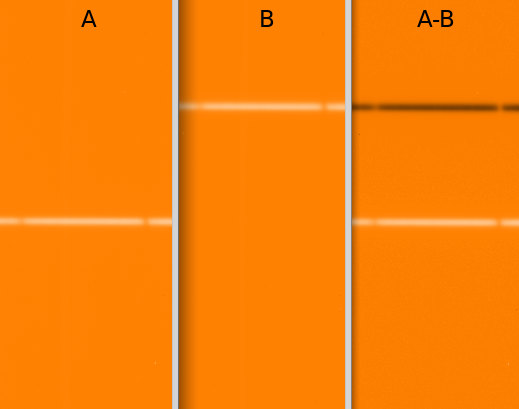
\includegraphics[width=0.4\textwidth]{figures/reduction/Nods_AB_A-B_labelled.png} & 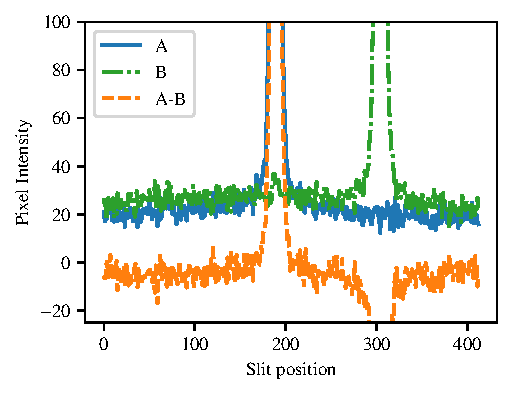
\includegraphics[width=0.42\textwidth]{figures/reduction/nod_slice_example.pdf} \\
    \end{tabular}
    \caption[Illustration of the nodding technique.]{Illustration of the nodding technique.
        Left: Sample slice of successive images at nod positions A and B, and their difference A minus B for detector \#1.
        Right: A vertical slice along the slit at column 512 (middle of detector).
        The background level observed in A and B is effectively removed by the subtraction.}
    \label{fig:nodimages}
\end{figure}

\subsection{\thar{} lamp calibration}
\label{subsec:th-ar}
As part of the {CRIRES} calibration procedure, spectra are taken of \thar{} lamps.
The \thar{} spectra are placed into the instrument using 6 optical fibres, creating six uniformly spaced spectra across the detector.
\cref{fig:caliblamps} contains the \thar{} spectra for all four detectors.
There are \(\sim50\) \thar{} lines that fall across the four detectors for the wavelength setting here, although most of them are faint.

The purpose of the \thar{} fibres is to perform cross-correlation against a \thar{} template to obtain a wavelength solution for each detector.
Optical defects (e.g.\ scratches on the detector) interfere with the performance of the correlation between \thar{} lines and the spectral template in {ESO} pipeline.
This can be resolved by first applying a pixel mask (although we did not attempt it).
At the top and bottom there are also two meteorological fibres that can not be used for wavelength calibration as they pass through a different optical pathway.
The brightest one at the bottom has strong features that seem to overwhelm or washout many columns in detector \#2--4 (vertical stripes).
This information is included here for completeness, as the \thar{} were not used in the chosen data reduction method, see \cref{subsec:wavecalib}.

%\begin{figure}
%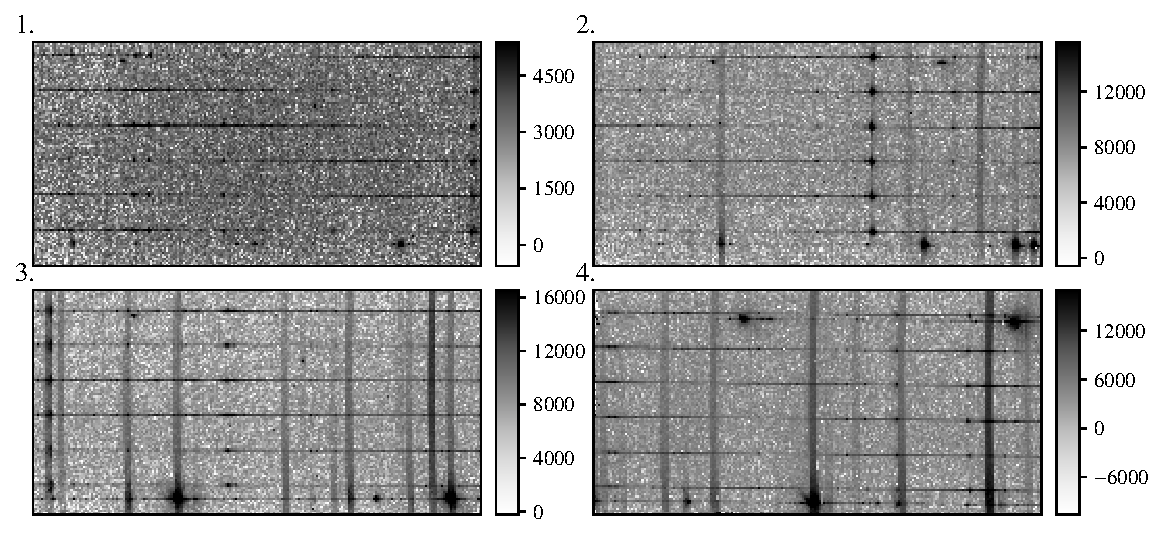
\includegraphics[width=\hsize]{./figures/reduction/lamp_plots_cbar_each.pdf}
%\caption[]{A \thar{} calibration lamp frame for each detector, corrected from the dark current.}
%  \label{fig:caliblamps}
%\end{figure}

\begin{figure}
    \begin{tabular}{cc}
         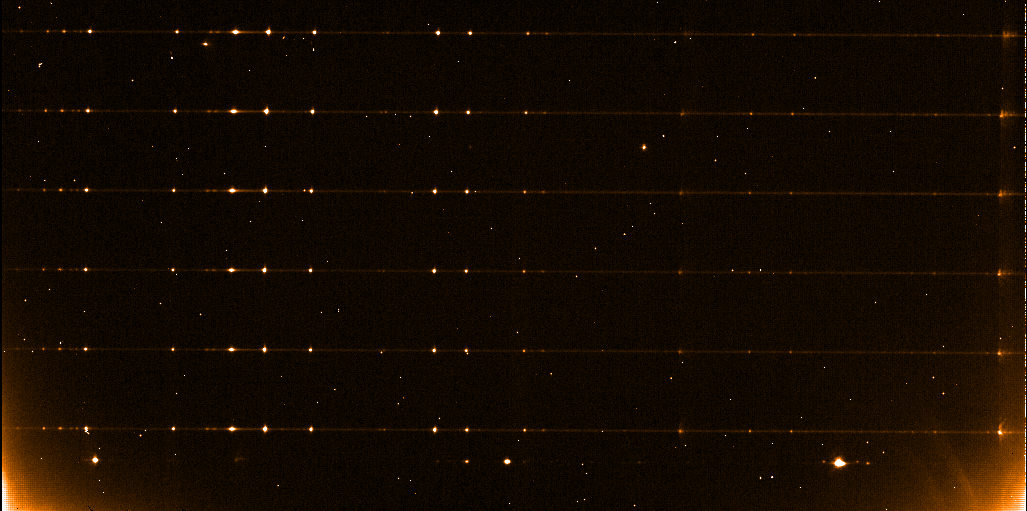
\includegraphics[width=.45\hsize]{./figures/reduction/Thar_1.png} & 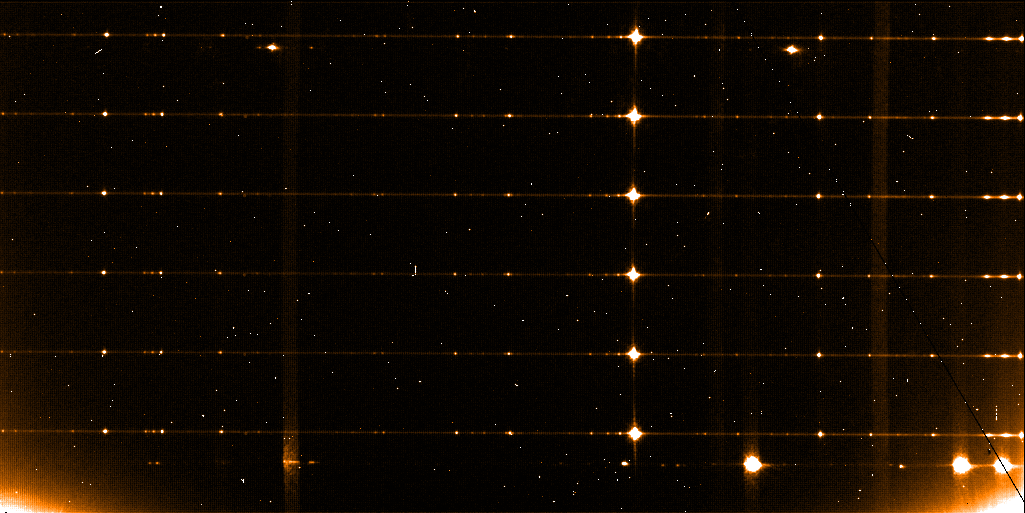
\includegraphics[width=.45\hsize]{./figures/reduction/Thar_2.png} \\
         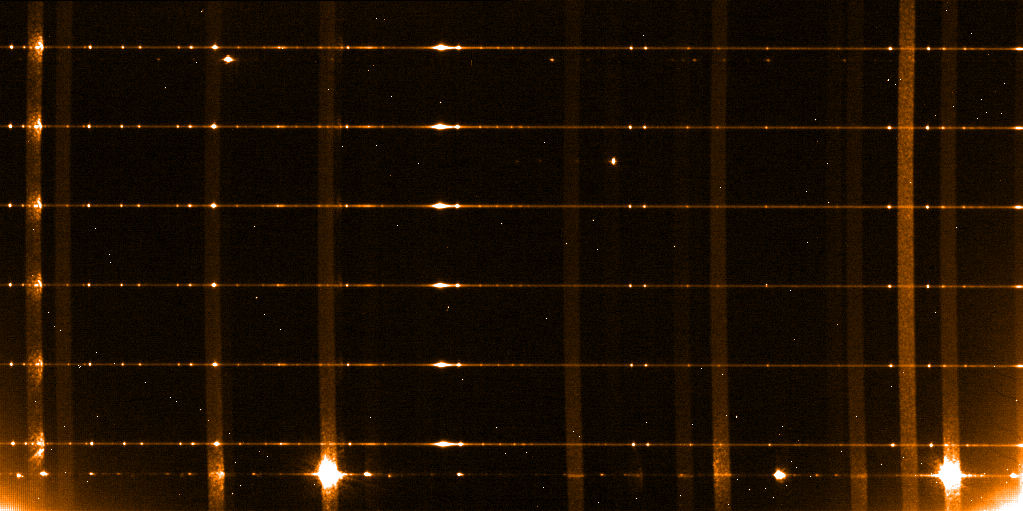
\includegraphics[width=.45\hsize]{./figures/reduction/Thar_3.png} & 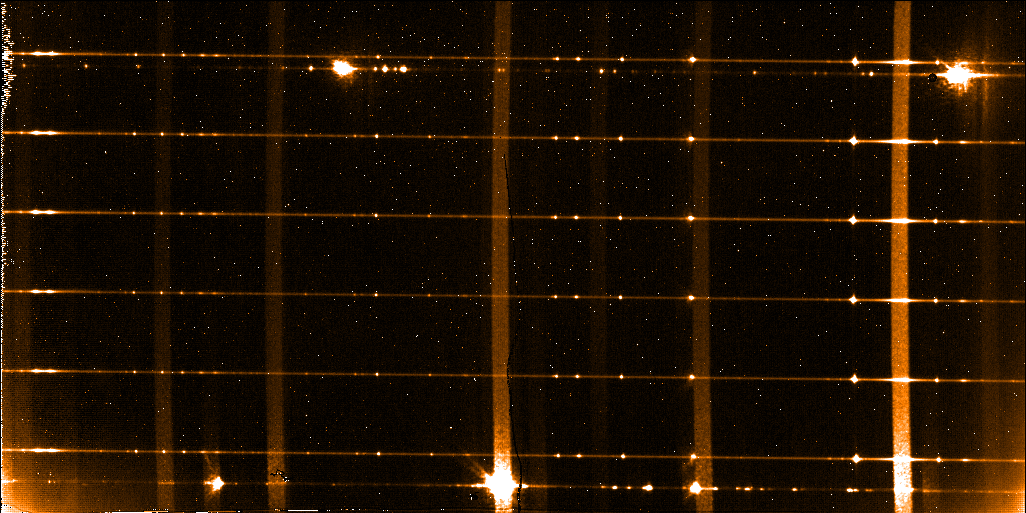
\includegraphics[width=.45\hsize]{./figures/reduction/Thar_4.png} \\
    \end{tabular}

    \caption[Example \thar{} calibration lamp frames for each detector.]{Example \thar{} calibration lamp frames for each detector.
        These are the raw frames in which dark current correction has not been performed (i.e the dark current is still visible on the bottom corners).}
    \label{fig:caliblamps}
\end{figure}


\subsection{Extraction}
\label{subsec:extraction}
The process of extraction is, in brief, turning the two-dimensional image of the spectrum into a one-dimensional representation.
This is done by summing the photon counts along the spatial direction, for each column in the dispersion direction in a small window around the spectrum.
To do this one needs to identify the position of the spectrum across the detector, referred to as {order tracing}.
In our case there is only one spectral order present but in a cross-dispersed configuration there can and will be many orders.
A rectangular box, with a specified aperture width, is centred along the traced spectrum.

There are two types of extraction commonly used.
The \emph{rectangular} extraction performs a simple aperture sum in the spatial direction, counting all photon counts that fall within the aperture.
An \emph{optimal} extraction~\citep{horne_optimal_1986} also includes variance weighting to reduce the impact of the noise and deviant pixels on the spectral extraction.
A spatial profile is fitted to the spectra and the pixels weighted such that the those furthest away from the centre have less impact on the sum.
Optimal extraction can increase the effective exposure time by up to 1.69 times at \(3 \sigma\)~\citep{horne_optimal_1986}.
Both rectangular and optimal extraction methods are available from both the {ESO} {CRIRES} and {DRACS} pipeline, compared below.


%!TEX root = ../../thesis.tex

\section{Pipeline Comparison}
\label{sec:pipelines}
To transform the observed 2-D image from the telescope into an extracted 1-D spectrum of the target a number of steps (some outlined above in \cref{subsec:nirreduction}) have to be performed in sequence.
The series of steps, performed by various software tools, is referred to as a \emph{pipeline}.
Each stage in the pipeline performs a specific task, for example creating the master dark frame, or performing the nod subtraction.
The result of one stage is passed to the next (either automatically or manually).
Two different pipelines were available to reduce the {CRIRES} observations used in this work.
The first is the standard {CRIRES} pipeline\footnote{\href{https://www.eso.org/sci/software/pipelines/}{https://www.eso.org/sci/software/pipelines/}}, available from {ESO}.
The second is an in-house pipeline previously used in~\citet{figueira_radial_2010} called {DRACS} (Data Reduction Algorithm for {CRIRES} Spectra)
This was created due to a lack of a reduction pipeline for CRIRES at the time.
In these next sections the experience gained using both pipelines, comparing the extracted spectra and user experience is documented.


\subsection{{ESO} {CRIRES} pipeline}
\label{subsec:eso-crires}
The {ESO} {CRIRES} pipeline was used to reduce {CRIRES} nodding spectra following direction from the {CRIRES} pipeline user manual\footnote{\href{ftp://ftp.eso.org/pub/dfs/pipelines/crires/crire-pipeline-manual-1.13.pdf}{ftp://ftp.eso.org/pub/dfs/pipelines/crires/crire-pipeline-manual-1.13.pdf}} and the {CRIRES} reduction cookbook\footnote{\href{https://www.eso.org/sci/facilities/paranal/instruments/crires/doc/VLT-MAN-{ESO}-14200-4032\_v91.pdf}{https://www.eso.org/sci/facilities/paranal/instruments/crires/doc/VLT-MAN-{ESO}-14200-4032\_v91.pdf}}.

The GASGANO\footnote{\href{https://www.eso.org/sci/software/gasgano.html}{https://www.eso.org/sci/software/gasgano.html}} graphical user interface (GUI) was used to interact with the pipeline with guidance from the {GASGANO} manual\footnote{\href{https://www.eso.org/sci/software/gasgano/VLT-PRO-{ESO}-19000-1932-V4.pdf}{https://www.eso.org/sci/software/gasgano/VLT-PRO-{ESO}-19000-1932-V4.pdf}}.
This pipeline provides a number of \emph{recipes} which perform the required extraction steps.
From the GUI each recipe is manually selected, then the correct calibration and observation files need to be selected to use with each recipe.
The final output from the {ESO} pipeline is a table in a fits format with the combined extracted spectra (both \emph{rectangular} and \emph{optimal} extractions), pixel errors and a wavelength solution.

For a novice of spectral extraction this pipeline and the available documentation was very helpful to get started and perform the extraction.
However, to reduce many spectra it soon became a long tedious process.

Constant revision of the documentation was necessary to ensure all the correct image and calibration files were added to each recipe.
The {ESO} pipeline makes all the recipe parameters easily accessible to modify via a window of the recipe interface, but the recipe parameter defaults get restored for each observation, making it difficult to reduce all of the observations in a consistent manner.
Having the parameters adjustment on the recipe interface is great for adjusting the parameters and for identifying which parameters are relevant to each recipe.
Unfortunately, when trying to experiment with the recipe parameters to achieve a high quality spectral extraction it was repetitive to change the same parameters for each observation, and it was also difficult to keep track of all the changes while assessing their effect on the final output.

The parameters for the wavelength calibration were the most tedious.
To try and improve the wavelength calibration, the {y-positions} of the 6 \thar{} fibres were manually found from the images for each detector and every observation and then entered as input parameters for the calibration recipe.
This helped the wavelength calibration recipe to correctly identify/fit more of the \thar{} spectra in most cases, but this took time.
Because of this, it was chosen to use the other pipeline and these calibration were not used.

{ESO} has a new reduction ``workflow'' called {ESO} Reflex~\citep{freudling_automated_2013}\footnote{\href{https://www.eso.org/sci/software/esoreflex/}{https://www.eso.org/sci/software/esoreflex/}}.
This enables automated reduction with the ability to chain together the extraction recipes in the specific order desired, repeat steps to optimize the reduction, and automatically handle the data organization (no need to manually select the files for each recipe).
This would likely have enabled a quicker and more consistent reduction of the spectra.
Unfortunately {ESO} Reflex was not, and is still not, available for the {CRIRES} pipeline.

\subsection{{DRACS}}
\label{subsec:dracs}
{DRACS} (Data Reduction Algorithm for {CRIRES} Spectra) is a custom reduction pipeline~\citep{figueira_radial_2010} written in {IRAF}'s CL\footnote{{IRAF} is distributed by the National Optical Astronomy Observatories, which are operated by the Association of Universities for Research in Astronomy, {Inc.}, under cooperative agreement with the National Science Foundation.}~\citep{tody_iraf_1993}.
It provides for automated dark and nonlinearity corrections (using the nonlinearity coefficients provided by {ESO}), as well as the flagging and replacement of bad pixels.
Sensitivity variations are corrected by dividing by a flat-field which was corrected from the blaze function effect.
The nodding pairs are mutually subtracted and the order tracing is accomplished by fitting cubic splines.
Order tracing allows the extraction algorithm to follow the shape for the dispersion across the detector\footnote{The spectra do not fall perfectly horizontally on the detector and usually contain some curvature due to the optics of the instruments.}.
By default the pipeline returns the \emph{optimal} extraction~\citep{horne_optimal_1986}, but the \emph{rectangular} extraction can also be obtained.
The extracted spectra from each nod is continuum normalized by dividing by a polynomial fitted to the continuum, with the polynomial degree selected individually for each spectrum and detector.
Finally, the normalized nod-cycle spectra are averaged together to give a single reduced spectrum, normalized to 1.

The {DRACS} pipeline was originally developed to work with \emph{H}-band spectra.
Because of this, some of the parameters were adjusted in an attempt to achieve a better reduction on the \emph{K}-band spectra analysed here.
The parameters adjusted were the tracing and normalization polynomial functions and their specific order on the detector.
Also, there was initially no reduction parameters present for the third detector as it was not reduced in previous works using this pipeline.
Therefore, the pipeline was extended to be able to reduce detector \#3 of CRIRES, by adjusting the pipeline code and finding suitable parameters for detector \#3.

When using the {DRACS} pipeline on a new target, the tedious part is initially creating the lists of files identifying which files are the dark, flat, and the science frames\footnote{The {GASGANO} {GUI} was helpful to identify the distinction of each fits file for a beginner.}.
After these lists are created, the reduction pipeline can be run and re-run easily, making the effort worth it.

The first time through is interactive with a number of manual checks and decisions to be made (e.g.\ confirming the order tracing position, and fit is good).
{DRACS} remembers choices in a database, allowing for a reduced level of user interaction a second or third time through the pipeline.
This was useful to experiment with and iterate the reduction parameters of the pipeline.
When changing the parameters which affect the order tracing, the database with the order tracing results needed to be deleted so that it would not influence the new fits.
These parameters were therefore slower to iterate on.

This semi-autonomous nature of the {DRACS} pipeline means that all the spectra can be reduced in a simple and consistent way, relatively quickly, and does not require manual spectra selection for each individual recipe as was done with the {ESO} pipeline.

There are a couple of drawbacks with using the {DRACS} pipeline.
The first is the lack of documentation on how to use it.
This required looking through the source code to find which functions and scripts do which part of the extraction.
{DRACS} makes use of many {IRAF} packages which have documentation available online\footnote{Such as at the \href{Space Telescope Science Institute}{http://stsdas.stsci.edu/gethelp/pkgindex\_noao.html}.}.
Searching through this documentation was difficult, but required, to understand how to use and modify {DRACS}.

The second drawback is that {DRACS} does not perform wavelength calibration, which is included with the {ESO} pipeline.
This means an external wavelength calibration was the only option (see \cref{subsec:wavecalib}).
The last drawback is the discovery of artefacts present in the nod spectra, which are discussed in detail in \cref{subsubsec:reductionartefacts}.

In opposition to the official CRIRES pipeline, {DRACS} allows for a simple way to do homogeneous reduction of data. However, this pipeline resorts to the {IRAF} recipes, which in turn have to be fine tuned in detail thorough extensive parametrization to reduce the data correctly.

\subsection{Pipeline comparison and selection}
\label{subsec:pipeline-selection}
\begin{figure}
    \begin{tabular}{cc}
        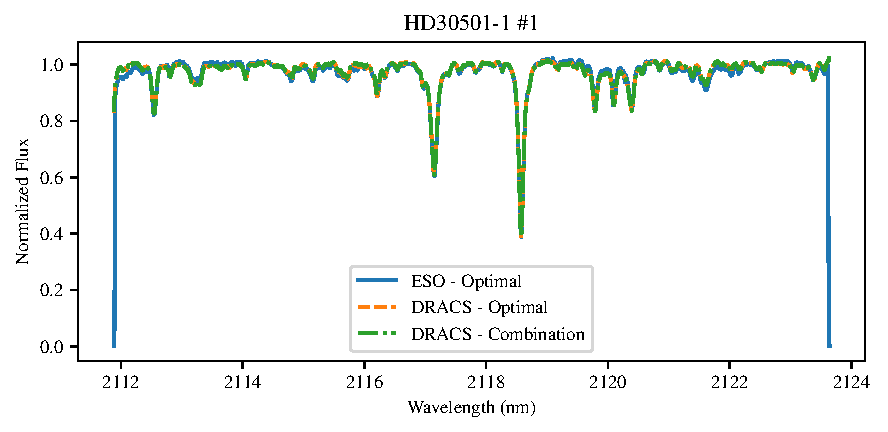
\includegraphics[width=0.47\linewidth]{figures/reduction/pipeline_compare/pipeline_compare_HD30501-1_chip_1} & 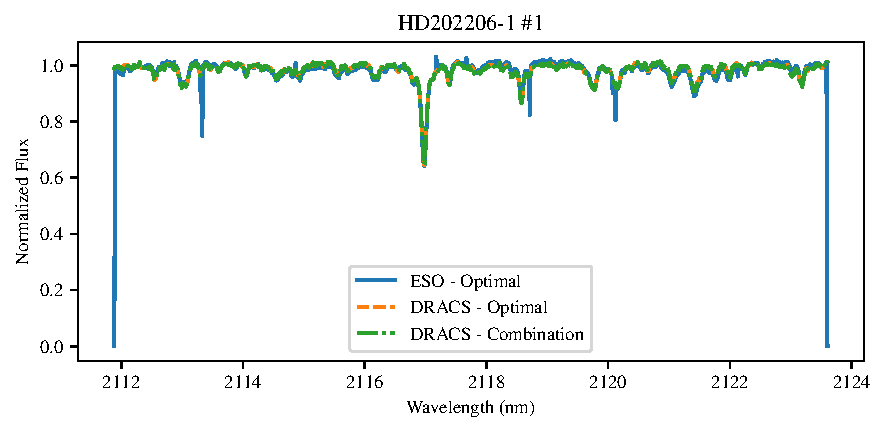
\includegraphics[width=0.47\linewidth]{figures/reduction/pipeline_compare/pipeline_compare_HD202206-1_chip_1}\\
        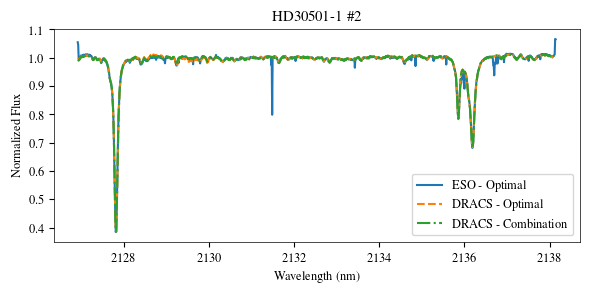
\includegraphics[width=0.47\linewidth]{figures/reduction/pipeline_compare/pipeline_compare_HD30501-1_chip_2} & 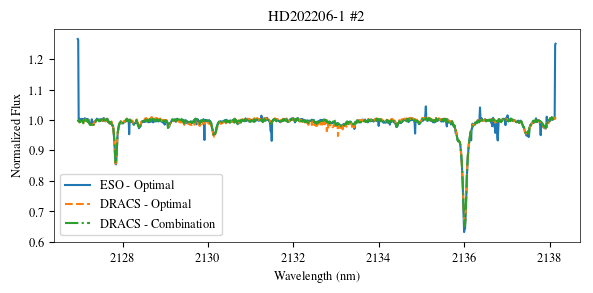
\includegraphics[width=0.47\linewidth]{figures/reduction/pipeline_compare/pipeline_compare_HD202206-1_chip_2}\\
        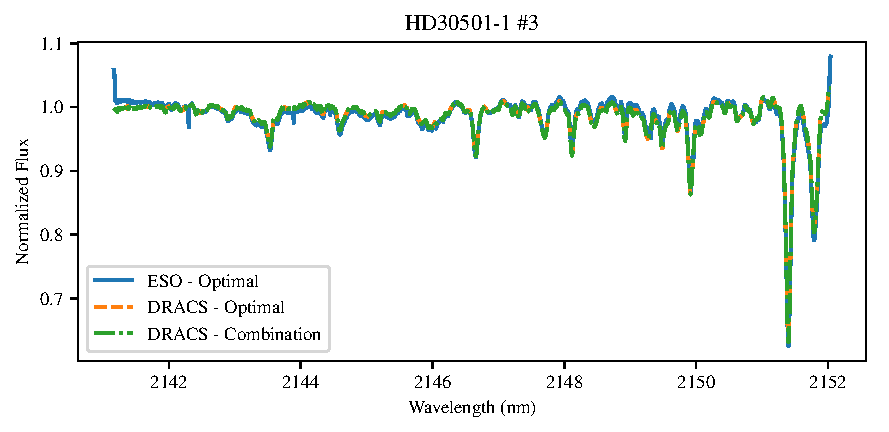
\includegraphics[width=0.47\linewidth]{figures/reduction/pipeline_compare/pipeline_compare_HD30501-1_chip_3} & 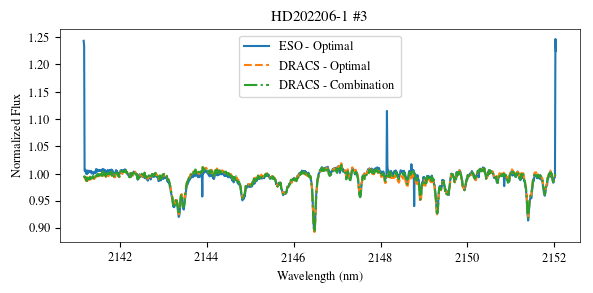
\includegraphics[width=0.47\linewidth]{figures/reduction/pipeline_compare/pipeline_compare_HD202206-1_chip_3}\\
        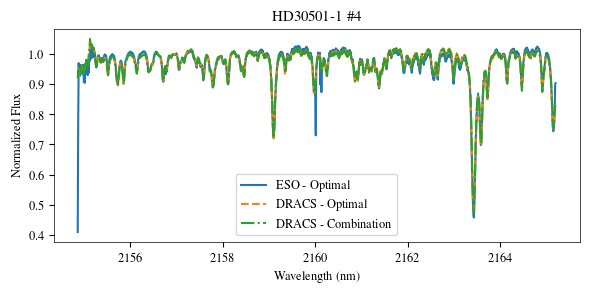
\includegraphics[width=0.47\linewidth]{figures/reduction/pipeline_compare/pipeline_compare_HD30501-1_chip_4} & 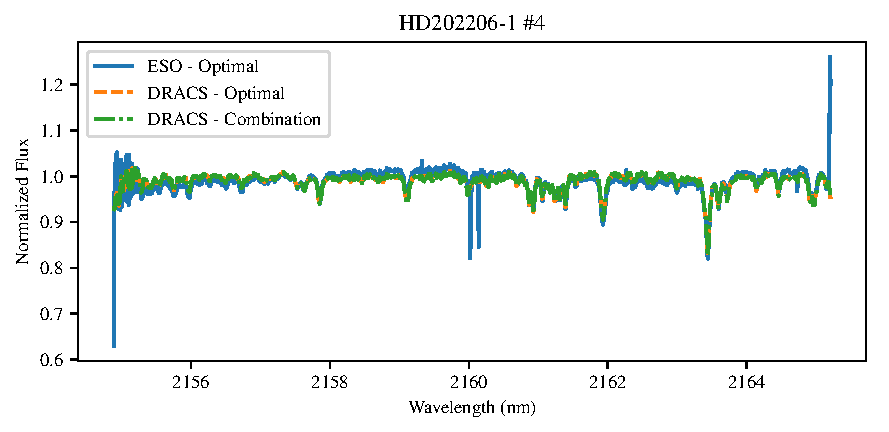
\includegraphics[width=0.47\linewidth]{figures/reduction/pipeline_compare/pipeline_compare_HD202206-1_chip_4}\\
    \end{tabular}
    \caption[Comparision between {DRACS} and {ESOs} reduction pipeline output.]{Comparison between the {ESO} pipeline and {DRACS} pipeline for two observations, {HD30501-1} and {HD202206-1}.
        The blue lines are the extracted spectra from the {ESO} pipeline, the orange dashed lines are the combined optimal extraction from the {DRACS} pipeline, and the green dash-dotted line is the modified {DRACS} extraction (after removing artefacts addressed in \cref{subsubsec:reductionartefacts}).
        The wavelength information applied to both spectra is from the {ESO} pipeline.}
    \label{fig:reduction-comparison}
\end{figure}

Both reduction methods were applied to the same {CRIRES} spectra to check the quality and consistency of both methods.
Two examples of the extraction for HD\,30501-1 (left) and HD\,202206-1 (right) from both pipelines are provided in \cref{fig:reduction-comparison}.
The blue lines are the extracted spectra from the {ESO} pipeline, the orange dashed lines are the optimal extraction from the {DRACS} pipeline, while the green dash-dotted line is the {DRACS} extraction after dealing with artefacts in the optimal extraction addressed in \cref{subsubsec:reductionartefacts}.

One of the important things checked was the line depths of each spectra to ensure that the pipelines were consistent.
The {ESO} pipeline has noticeable issues, with many large spikes still present in the spectra, likely caused by bad pixels or cosmic rays that are not correctly removed.
There also appears to be problems with the edges of the {ESO} reduced spectra, with very large spikes at either end.

At this stage the {DRACS} pipeline was chosen, as it was considered that the {DRACS} pipeline produced better extracted spectra than the {ESO} pipeline.
This decision was based on the quality of the reduced spectra, as well as the relative ease of use of the pipeline (being semi-automated once set up).
Another deciding factor was the need to create software to remove the bad pixels observed in the {ESO} reduced spectra.
However, this was unavoidable as it was eventually required for the {DRACS} reduced spectra (see \cref{subsubsec:reductionartefacts}).
Though the {ESO} pipeline provided a wavelength solution for the spectra, this did not factor into the decision as it was considered too unreliable due to known issues with {CRIRES} wavelength calibration, necessitating a new wavelength calibration anyway.

The spectra for the pipeline comparison in \cref{fig:reduction-comparison} are the combination of the 8 nod spectra.
Later, it was discovered that individual nod spectra from the {DRACS} pipeline had issues (see \cref{subsubsec:reductionartefacts}).
These are difficult to notice on this scale as they each constitute one eighth of the information in the combined spectrum.
An example of this is seen in detector \#2 of {HD202206-1} in \cref{fig:reduction-comparison}.
In \cref{fig:resizednods} an artefact from a single nod spectra, is barely visible in the pipeline comparison of \cref{fig:reduction-comparison}, shown as a slight depression of the orange dashed line between 2\,132 and 2\,134\nm{}.
The identification of these artefacts and how they are removed (green lines) are explained in the following section.




%!TEX root = ../../thesis.tex

\subsubsection{Reduction issues}
\label{subsubsec:reductionartefacts}
After the decision to use the {DRACS} pipeline large artefacts in the {DRACS}-extracted spectra were observed.
An investigation into the cause of these artefacts was undertaken to identify their source and attempt to remove them from the spectra.
The eight individual nod spectra were displayed side-by-side which revealed that occasionally the spectra from one of the nods deviated significantly from the others.
Eventually it was identified that the artefacts were only in the \emph{optimally} reduced spectra, and that they were not present in the \emph{rectangular} extracted nods.
An example is shown in \cref{fig:artefact_example_hd162020} in which sharp spikes in the middle panel (rectangular extraction) correspond to deviations observed in the top panel (optimal extraction).
The bottom panel shows the difference in the combined average spectra from the optimal extraction and the corrected mixed spectrum resulting from the method given in this section to remove the artefacts.
In this case the deviation in the combined spectra are at 2\%.
Further visual examples of artefacts, selected to show a variation in appearance, are given in \cref{appendix:artefacts} along with a table identifying the observations and nod spectra the artefacts were observed in.


\begin{figure}
    \centering
    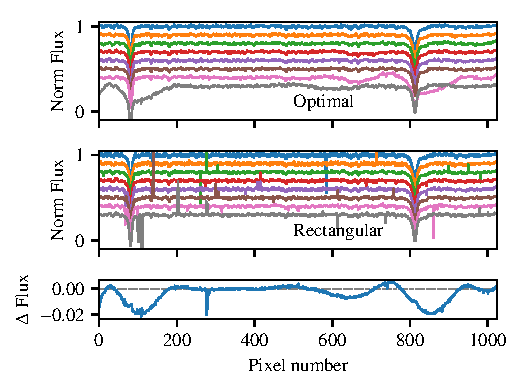
\includegraphics[width=0.7\linewidth]{figures/reduction/bp_plots/extraction_comparision_HD162020-1_chip_2.pdf}
    \caption[Example of {DRACS} artefacts in the optimally extracted spectra {HD\,162020}.]{Example of {DRACS} artefacts in the optimally extracted spectra second detector of the first observation of {HD\,162020}.
        top: The 8 normalized nod spectra obtained using \emph{optimal} extraction, vertically offset from each other.
        middle: The 8 normalized nod spectra obtained using \emph{rectangular} extraction, vertically offset from each other.
        bottom: Difference between the combined average spectra from the top and improved result from the mixed method developed here.
        The middle panel creates the small spikes, while the large deviations are due to the artefacts in the optimal reduction.
        There are three bad pixel spikes that cause artefacts in this optimal extraction.
        These are located in the seventh nod (pink) around pixel 850, and two in the eight nod (grey) around pixel 100 and 620.
        Several other spikes do not cause any artefacts in the optimal reduction.}
    \label{fig:artefact_example_hd162020}
\end{figure}

%\textbf{
%    EXAMPLE with the new-old \cref{fig:badpixelreplacement}}.
%\todo{CHANGE the figure here}
%\begin{figure}
%    \centering
%    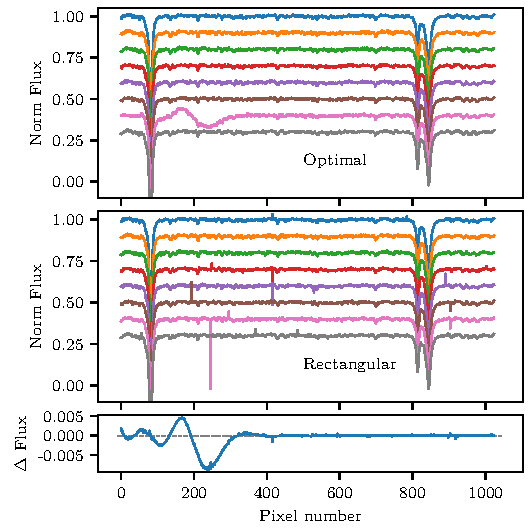
\includegraphics[width=\hsize/2]{figures/reduction/bp_plots/Bad_pixel_replacement}
%    \caption[]{Example of an artefact in the optimally extracted spectra from detector \#2 of {\red{} HDXXXXXX}.
%        The top panel contains the 8 normalized nod spectra obtained using optimal extraction.
%        The middle panel shows the same nod spectra reduced using only rectangular extraction.
%        The bottom panel shows the difference between a combined spectrum using optimal nods only and a combined spectrum in which the identified nods are replaced with their rectangular counterparts as per \cref{subsubsec:reductionartefacts}.
%        A vertical offset is included between each spectra for clarity.
%        The nod spectra are in observation order from top to bottom.}
%    \label{fig:badpixelreplacement}
%\end{figure}

It is clear that the artefacts in the optimal extraction occur when there is a corresponding ``bad-pixel'' spike\footnote{Their exact origin is unknown but are likely uncorrected bad-pixels or a cosmic ray.
Here they will be referred to as bad-pixels.} in the rectangular extraction.
However this is not always the case with many spikes observed (e.g. first nod around pixel 580 in \cref{fig:artefact_example_hd162020}) that are automatically removed in the optimal extraction.
The occurrence of artefacts in the observations did not appear to have a pattern with nod position or detector with 14\% (79/544 spectra) of the nod spectra having an optimal exaction that seemed to misbehave.
The artefacts in the optimal extraction are also largely extended, significantly affecting more of the spectrum that the individual spikes (up to 100s of pixels).
Artefacts were observed arising from both large and small spikes alike while other large and small spikes are removed.
This possibly suggests that their size is of less importance, that some other unknown factor (possibly location).

As mentioned in \cref{subsec:extraction} the \emph{optimal} extraction includes variance weighting across the spatial direction.
It appears that the presence of the bad pixel spikes heavily affects the variance weighting procedure during the \emph{optimal} extraction.

Numerous parameters in the {DRACS} pipeline were experimented with in the attempt to remove the observed artefacts with limited success.
For instance, no complete removal of the artefacts was found by adjusting the \(\sigma\) rejection limits (between \(1-5 \sigma\)) or  increasing the tracing width parameter in {IRAF}s DOSLIT\footnote{Documentation for DOSLIT can be found here \href{http://stsdas.stsci.edu/cgi-bin/gethelp.cgi?doslit}{http://stsdas.stsci.edu/cgi-bin/gethelp.cgi?doslit}} recipe, although they did slightly affect the shape of the artefacts.
\cref{fig:resizednods} shows the extraction of HD\,202206 with one parameter changed in the reduction pipeline.
The only difference between the left and right panels the automated aperture resizing\footnote{Using \href{apresize}{http://stsdas.stsci.edu/cgi-bin/gethelp.cgi?apresize.hlp}} was enabled by setting the ``resize'' parameter to \emph{yes} in the right hand panel.
This manages to remove an ugly artefact in the sixth nod (brown), but not the artefact in the seventh nod (pink).
This was only discovered in the writing of this thesis so could not be utilized earlier.
However, it does indicate that some improvements may be obtained with extensive time and patience tweaking the parameters of the {DRACS} pipeline.

\begin{figure}
    \centering
    \begin{tabular}{cc}
        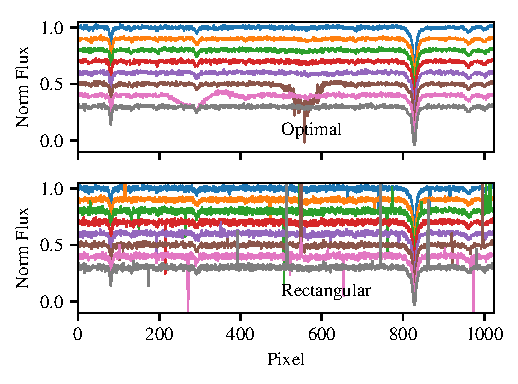
\includegraphics[width=0.5\linewidth]{figures/reduction/bp_plots/non_resized_nods_HD202206-1_chip_2} & 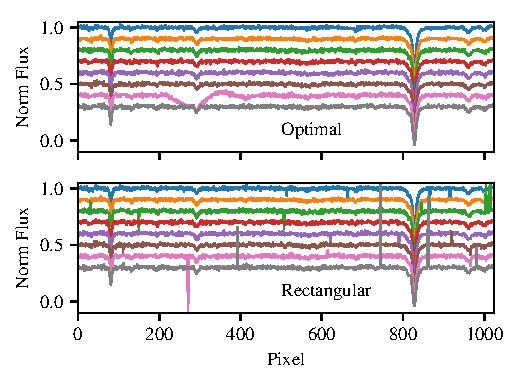
\includegraphics[width=0.5\linewidth]{figures/reduction/bp_plots/resized_nods_HD202206-1_chip_2}\\
    \end{tabular}\label{fig:resizednods}
    \caption[Artefacts comparision with and altered pipeline parameter.]{Two {DRACS} reductions for detector \#2 of HD\,202206-1 with one pipeline parameter changed.
        Left: The reduction with the {DRACS} pipeline with the ``doslit.resize'' set to ``no''.
        Right: The reduction from the same pipeline but with ``doslit.resize'' set to ``yes'', all else equal.
        During the order tracing the aperture size is automatically adjusted while the rest of the parameters remain identical.
        One large artefact is removed in the sixth nod (brown) while the artefact in the seventh nod (pink) is not removed.}
\end{figure}

The purpose of these observations was to detect faint companion spectra with expected flux ratios \(\rm {F_2}/{F_1} < 1\%\).
As the artefacts created large and extended deviations in the combined spectra (up to 2\%) measures were needed to remove these artefacts from the combined spectra.
To avoid contaminating the spectra of the faint companions.

After the unsuccessful tweaking of parameters the solution that was chosen was to replace the optimally extracted nods that contained artefacts with their rectangular counterparts.
This would create a combined spectra that had a mix of optimally reduced and rectangularly reduced nod spectra, without any artefacts.
To replace the spikes in the rectangular extraction that created the artefacts and others an iterative 4-\(\sigma\)\footnote{There is no scientific justification why 4-\(\sigma\) was chosen over the commonly used 3-\(\sigma\).} rejection algorithm\footnote{Found at \url{https://github.com/jason-neal/nod_combination}} was applied to the rectangular extractions.
The \(\sigma\) for each pixel was calculated as the standard deviation of the nearest 2 pixels on either side of it, across all 8 nod spectra (a $5\times8$ grid).
Any rejected pixels were replaced using linear interpolation along the spectra.
The spectra that contained artefacts and that were replaced using this method are given in \cref{tab:nod_replacement}.

Combined spectra were finally constructed by averaging the eight nod-cycle spectra together, where some of the optimally extracted spectra were replaced using the above method.
The actual spectra from the two different methods can be seen in \cref{fig:reduction-comparison} where orange is the combination of optimally reduced spectra only and green uses the replacement method outlined here.
The easiest to notice a difference is {HD\,202206-1 \#2} in which the artefacts from \cref{fig:resizednods} are removed.

The continuum normalization of the spectra is performed in {IRAF} while the swapping of nods creating a mixed combination is carried out in \emph{Python} along with the post reduction procedures detailed below.

The {DRACS} pipeline was originally chosen over the {ESO} {CRIRES} pipeline because it seemed relatively simpler to use, being semi-automated, and appeared to have less bad pixel/cosmic ray artefacts in the resulting spectra.
In hindsight the {DRACS} pipleline had several unexpected challenges due to these artefacts which took time to investigate and find a solution for.

One hypothesis for these artefacts is detector glow, the heating of the detector by the nearby amplifiers in the chip (see \cref{subsubsec:darkcurrent}.
The artefacts in the \emph{K}-band spectra were not observed in previous works in the \emph{H}-band using this pipeline~\citep[e.g.][]{figueira_radial_2010}, and as such may have a wavelength dependent effect, like detector glow.
However, it seems plausible that a glow related effect would be spatial distributed like the glow shown in \cref{fig:darkcurrent_colour}, but the location of the artefacts do not seem to have a discernible pattern.
It could also be that there were artefacts in intermediate steps of the previous works that were missed due to the semi-automated pipeline, with the resultant combined spectrum being only slightly affected at the level of >1\% it could easily be missed (e.g. \cref{fig:reduction-comparison}).
Anther possibility is that the artefacts are bad pixels not removed correctly.
Regardless, in the end they do not have a significant impact on the results found in this work, though it is expected that mixing the optimal and rectangular extracted spectra will have a slight negative impact on the noise or \snr{} of the combined spectrum.
Much time and effort was invested attempting to extract the spectra, without artefacts, to have the best chance at obtaining high quality scientific results of the faint features sought after in this work.



\subsection{Reduction experience:}
\label{subsec:experience}
The experience gained in reducing {CRIRES} spectra enabled participation in collaboration with other science cases.
The {DRACS} pipeline was used to extract the spectra of two other targets.
A target and a very brief aim of each science case is given below.
\begin{itemize}
\item Barnard's Star\footnote{Programme {{ID}}: 085.D-0161(A)}: The carefully reduced \nir{} spectra of Barnard's Star was meant to extend the work of~\citet{andreasen_nearinfrared_2016} in deriving the spectroscopic parameters of cool M-stars in the \nir{}.
Unfortunately the work did not advance enough to analyse M-star's and a spectrum of {Arcturus} (K0) and a fully reduced spectrum of {10Leo} (K1) from the {CRIRES}-POP library~\cite{nicholls_crirespop_2017} were analysed instead in~{Andreasen et al. (in prep.)}.
\item \(\eta\) Tel\footnote{Programme {{ID}}: 083.C-0759(A)}: The spectra of a telluric standard star (HIP100090) and {HR\,7329-B} (\(\eta\) Tel-B) a rapidly rotating Brown Dwarf, were reduced to accurately determine the BD rotation rate by measuring the line broadening.
The results from this data will be published in an upcoming paper {Hagelberg et al. (in prep.)}.
\item The same spectra of {HR\,7329-B} were also used in~\citet{ulmer-moll_telluric_2018} to compare different telluric correction methods in the \nir{}.
An example from~\citet[][(B.3)]{ulmer-moll_telluric_2018} of the reduced target spectrum (black), the telluric model () and the telluric corrected spectrum (green) is provided in \cref{fig:ulmermol2018tellcorrcrires48}.
\end{itemize}

\begin{figure}
    \centering
    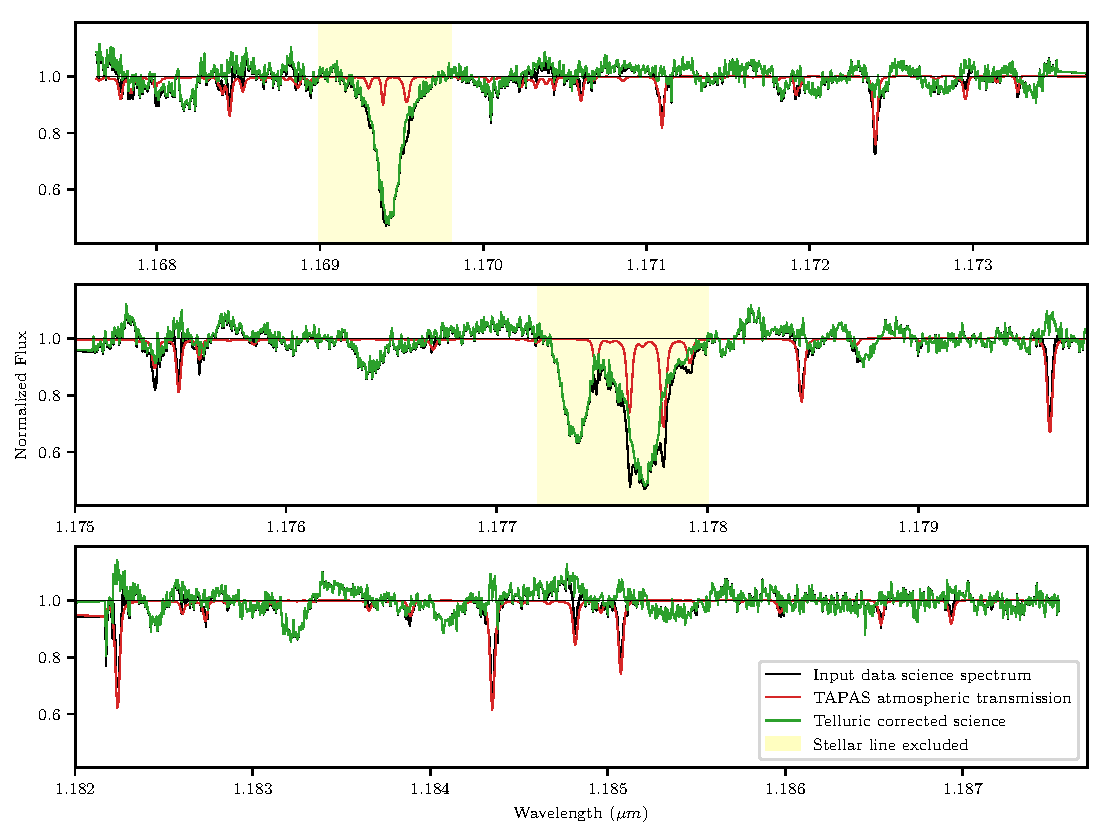
\includegraphics[width=0.7\linewidth]{figures/reduction/ulmermol2018_tell_corr_CRIRES_48}
    \caption[Example of telluric corrected spectrum of {HR\,7329-B} using {TAPAS}.]{Example of telluric corrected spectrum of {HR\,7329-B} using {TAPAS}.
Credit~\citet[][]{ulmer-moll_telluric_2018}.
The yellow shaded region is the region of stellar lines that was avoided while applying the correction methods.}
    \label{fig:ulmermol2018tellcorrcrires48}
\end{figure}

For these works only the spectral extraction outlined above was performed.
The post extraction and reduction steps detailed in the following sections were not.


%!TEX root = ../../thesis.tex

\section{Post reduction stages}
\label{sec:posreduction}
From the {DRACS} pipeline the 1-D spectra of each target has been extracted.
However, the spectra still need to undergo some post-extraction steps.
In particular, wavelength calibration and telluric correction.
A detailed look of how these steps were developed and performed are addressed in the following section.

\subsection{Wavelength calibration}
\label{subsec:wavecalib}
Wavelength calibration is the process of assigning accurate wavelength values to each pixel in the spectra.
For {CRIRES} in the \nir{} this is challenging.
{CRIRES} uses a Thorium-Argon (\thar) lamp to place 6 emission spectra on the detector using fibres.
The spectra of the \thar{} emission lines are used to determine the spatial distribution of the wavelength solution across each detector using correlation with a spectral template.
\thar{} lamps are excellent at optical wavelengths where the numerous (several thousand) spectral lines enable precision of sub\,-\mps{} radial velocity measurements {HARPS} spectrograph.

However, in the \nir{} there is a relatively low density of \thar{} lines~\citep{kerber_laboratory_2009}, which, in combination with the alignment of the narrow wavelength range of the detector, causes a poor wavelength calibration to be obtained (e.g.\ {CRIRES}-POP~\citep{nicholls_crirespop_2017}).
Above 2.2\um{} there are {O-H} sky lines that can be used for wavelength calibration but according to the {CRIRES} manual for observations below 2.2\um{} they are too dim.
These wavelength calibration issues were experienced when using the {ESO} {CRIRES} pipeline, with non-\thar{} features sometimes affecting the correlation.

Between the wavelength range 2.1--2.17\um{} there are roughly 80 \thar{} lines across all four detectors, as seen in \cref{fig:caliblamps}.
The {DRACS} pipeline does not use the \thar{} lamp files for wavelength calibration and leaves this as a post reduction step.

A common method for wavelength calibration that does not rely on \thar{} lamps of {CRIRES} involves using the telluric lines present to provide the wavelength solution~\citep[e.g.][]{brogi_signature_2012,brogi_carbon_2014,dekok_detection_2013,piskorz_evidence_2016}.
This is made possible by the use of high resolution spectra, in which the telluric lines are well resolved, as well as accurate spectral information of the atmosphere.

Likewise, in this work the wavelength calibration is performed using the telluric absorption lines present in each observation as the wavelength reference.
Instead of directly using the {HITRAN} database~\citep{rothman_hitran2012_2013} for the telluric line positions, such as~\citet[][]{brogi_signature_2012, brogi_carbon_2014, dekok_detection_2013}, use the {TAPAS} atmospheric transmission models (see \cref{sec:telluric_correction}).
The {TAPAS} models use the {HITRAN} database but also includes atmospheric profiles and physical meteorological measurements to model the telluric absorption strength.

To calibrate the wavelength the telluric lines in the model need to be associated to the corresponding telluric lines in the observed spectrum.
The centroid\footnote{Centre of the line} of each telluric line in the model is obtained by fitting the telluric transmission spectrum, \(T(\lambda)\), as a simple sum of Gaussian functions (subtracted from the continuum):
\begin{equation}
T(\lambda) = 1 - {\Sigma}_{i}\ G(\lambda, A_{i}, {\mu}_{i}, {\sigma}_{i}),
\end{equation}
where \(G\) is a Gaussian function of the form
\begin{equation}
G(\lambda, A, \mu, \sigma) = {A \textrm{e}}^{{-(\lambda-\mu)}^{2}/2\sigma^{2}},
\end{equation}
and \(A\), \(\mu\), \(\sigma\) are the amplitude, central wavelength, and standard deviation for each line respectively.
Telluric lines actually have a Voigt profile\footnote{A Voigt profile is a convolution of two broadening profiles, a Gaussian and a Lorentzian.
Gaussian broadening results from thermal Doppler broadening, and instrumental broadening while the Lorentzian broadening comes from molecular vibrational bands\citep{meier_art_2005}.} although they are not fully resolved in the \nir{} and their shape is dominated by the instrumental profile.
\citet{seifahrt_synthesising_2010} measured the instrumental profile of {CRIRES} using singular-value decomposition and showed that it is extremely well represented by a single Gaussian below a \snr{}$\sim$300.
Therefore, wavelength calibration using single Gaussian fits to each line is sufficient.

The observed spectra contain two different spectral components: stellar and telluric lines, which are multiplied together: The observed spectra are therefore fitted with a multiplication of two Gaussian-sum models.
\begin{align}
I_{obs}(x) &= {I}_{tell}(x) \times {I}_{star}(x) \nonumber\\
I_{obs}(x) &= {\Big(1 - {\Sigma}_{j}\ G(x, A_{j}, {\mu}_{j}, {\sigma}_{j})\Big)}_{tell} \times {\Big(1 - {\Sigma}_{k} G(x, A_{k}, {\mu}_{k}, {\sigma}_{k})\Big)}_{star}, \label{eqn:obs}
\end{align}
where \(x\) is the pixel coordinates of the extracted spectra.

The identification between telluric and stellar lines is performed by hand for each spectra, using the telluric model as the reference.
Care was taken to fit the correct components to blended spectra where possible to improve the number telluric lines use for calibration.
The fits were inspected to ensure that they reasonably matched the line positions.
There was difficulty in identifying the shallow lines with depths below 1--2\%, but these were needed in some spectra to obtain a suitable fit.
If there were blended lines that did not appear to fit correctly they were not considered in the calibration step.

After fitting \(I_{obs}(x)\) to the observed spectrum and \(T(\lambda)\) to the telluric model, the wavelength solution was obtained by fitting a second order polynomial to the centroid values \(\{\mu_{j}(x), \mu_{i}(\lambda)\}\) from the telluric components of the observed spectra and telluric model respectively.
A second order polynomial has been shown to be sufficient for higher precision {RV} studies~\citep[e.g.][]{bean_groundbased_2010, figueira_radial_2010}.
This polynomial is then used to map the whole spectrum from pixels into wavelength.
Higher \(3^{\textrm{rd}}\) and \(4^{\textrm{th}}\) order polynomials that are also used in the literature~\citep[e.g.][]{seifahrt_synthesising_2010, ulmer-moll_telluric_2018} were attempted but had limited success here due to the limited number and uneven spacing of telluric lines in the narrow wavelength range analysed, especially on the second detector.
There were often large deviations due to the uneven spread of telluric lines, especially at the extremities.
Higher order terms for wavelength calibration are usually used in regions with a higher density of telluric lines and/or a longer wavelength span~\citep{piskorz_evidence_2016, seifahrt_synthesising_2010, ulmer-moll_telluric_2018}.

\begin{figure}
    \centering
    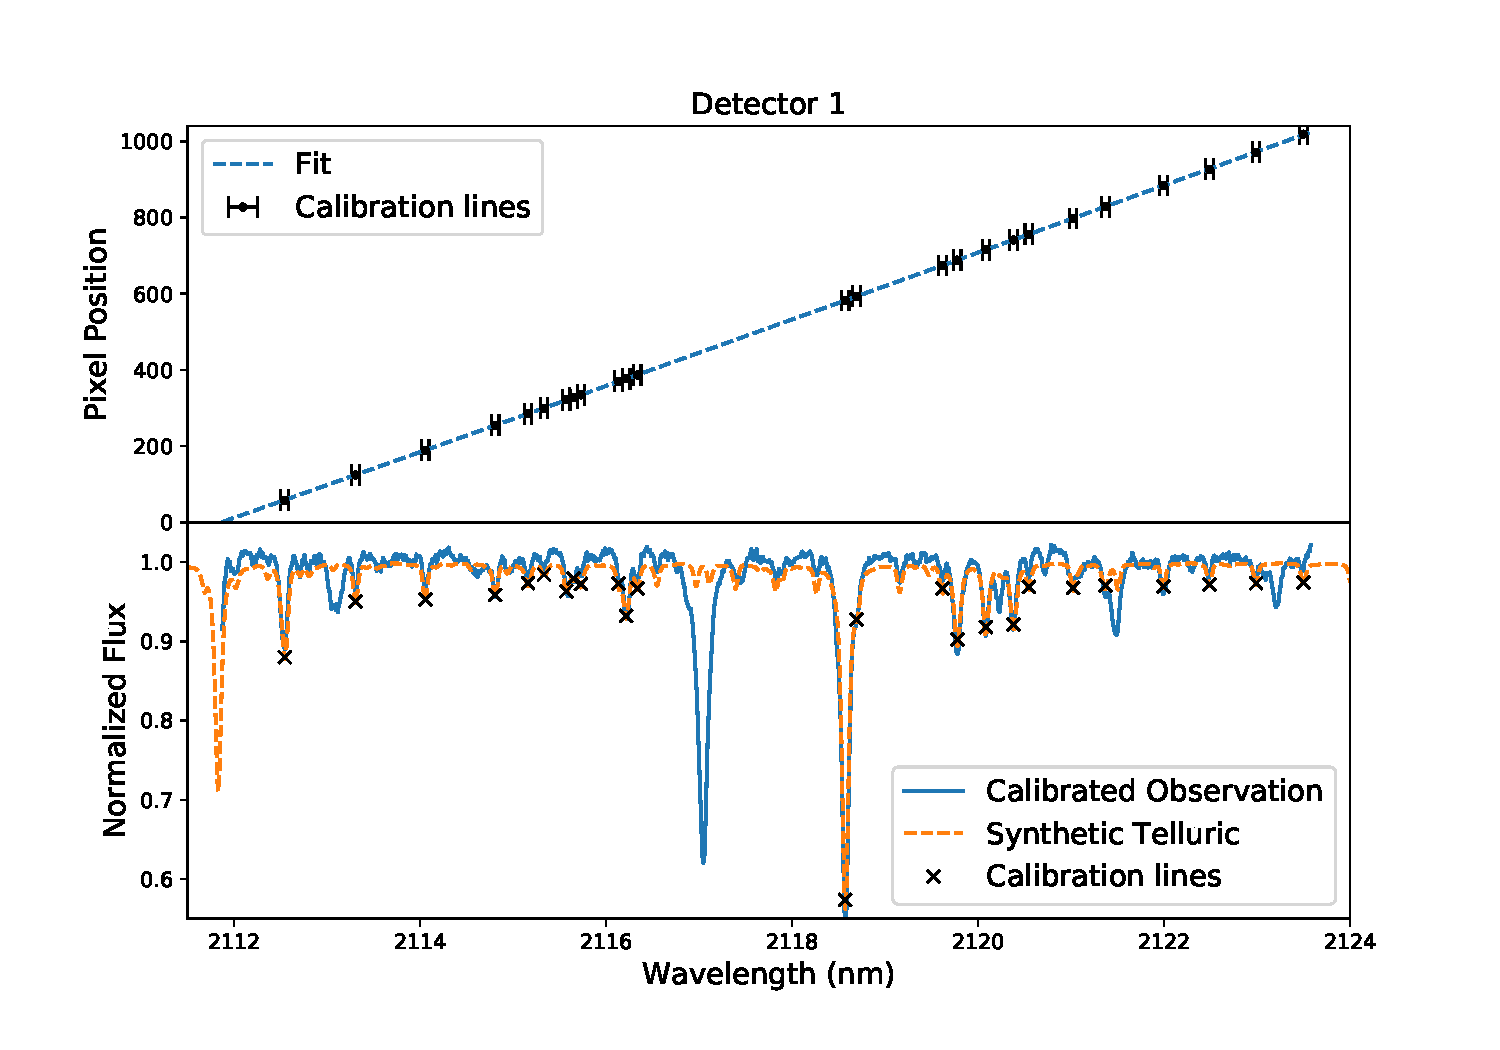
\includegraphics[width=0.8\linewidth]{figures/reduction/calibration.pdf}
    \caption[Example of the wavelength calibration using the synthetic telluric spectra.]{Example of the wavelength calibration using the synthetic telluric spectra.
        Top: The pixel/wavelength mapping and associated wavelength fit.
        The horizontal error bars shown are the Gaussian line width, around 0.04\nm{}.
        Bottom: The wavelength calibrated observation and the telluric model used for calibration.
        The black crosses indicate the peaks of the telluric lines used in the fitting process.}
    \label{fig:wl_calibration}
\end{figure}

An example of the wavelength fitting is given in \cref{fig:wl_calibration}.
The top panel shows the (slightly) quadratic fit (blue dashed) to the centroid values \(\{\mu_{j}(x), \mu_{i}(\lambda)\}\)(black) while the bottom panel shows the newly calibrated observation alongside the telluric spectrum.
The black crosses indicate the lines used for calibration.
To two decimal places the equation of the fit $\lambda = -1.85e^{-7} x^2 + 1.16e^{-2} x + 2111.86$.

Much like with the \thar{} calibrations, this technique performs better when there is sufficient coverage of telluric lines on the detectors.
For the wavelength setting of these observations, the spectra from the second detector (top right panel of \cref{fig:spectraexamples}) only has two large telluric lines present with several small lines, with relative depths smaller than 1\%, which are often difficult to accurately identify.
This deteriorated the calibration stability for the second detector.
The second detector may have been ideal for the detection of a faint secondary spectra, with the lack of telluric contamination and stellar lines.
Unfortunately the wavelength calibration quality varies in an inverse way, being more difficult with few lines.

It is noted that there are many variations on this wavelength calibration technique including those integrated within programs such as \emph{TelFit}~\citet{gullikson_correcting_2014}, and {ESO}'s \emph{Molecfit}~\citet{smette_molecfit_2015}, that perform telluric correction and re-calibrate the wavelength axis themselves at the same time.
It is recommended to attempt using those first before independently creating wavelength calibration software.

One improvement could have been to include a concurrent fitting of a stellar spectral model, adjusted for {RV}, along with the telluric model, which could help to improve the wavelength calibration performed here.
\citet{piskorz_evidence_2016} performed wavelength calibration using only a telluric line model at other \nir{} wavelengths (\emph{L}-band between 3.0--3.4\um{}) successfully.
However, around 2\um{} they needed to include a fitted stellar model to obtain good wavelength calibration due to the weaker telluric lines in this region.
This is the same wavelength region of the data analysed here.
Having experience of performing wavelength calibration at other wavelengths may have revealed the difficulties of calibration from the telluric lines at 2\um{} sooner.

A brief attempt of wavelength calibration using the iterative calibration method outlined in~\cite{brogi_rotation_2016} was made.
This involved generating a set of quadratic wavelength solutions for the observed spectrum and cross-correlating each one against the telluric model.
The solutions for the next iteration are obtained by refining the parameters from the wavelength solution with the highest correlation.
The method worked well for~\citet{brogi_rotation_2016} as they included templates for both the star and telluric lines and they were observing in a wavelength domain in which there is a large number of strong and uniform stellar \ce{CO} lines across the detector.
The brief experiments with this method were not successful as they did not include a stellar model or mask, which lead to incorrect fitting solutions.
Without adding any stellar masking the telluric lines would strongly correlate to the stellar lines present, especially where there were blended lines.
This lead to visibly incorrect wavelength solutions and this method was abandoned.
If a stellar mask was used it may have been possible to achieve more sensible results, although still challenging to the low density of telluric lines at this wavelength range.

At one point it was considered to attempt a global fit of the wavelength calibration, using all four {CRIRES} detectors together.
This would create a consistent fit to the dispersion across all 4 detectors at once.
This would require extra fitting parameters to define the size of the 3 gaps between the detectors and any vertical offsets.
This fit may even need to be performed on the two-dimensional images, before the 1-D extraction.
This may have allowed for the telluric lines from neighbouring detectors to help fit the calibration on detectors where there are very few telluric lines (e.g.\ detector \#2).
The fitted instrument parameters such as the detector gaps may even be constrained so that they are physically consistent across all observations.
However, this idea was not explored further or implemented due to time constraints.
An example of the wavelength calibration using all four detectors is provided in \cref{appendix:wavelength_fitting}.
In the future it may be possible or necessary to combine all of the methods above, including the \thar{} calibration lines, telluric models, stellar templates, and multiple detectors fitted at once to achieve precise wavelength calibration.

\begin{figure}
    \centering
    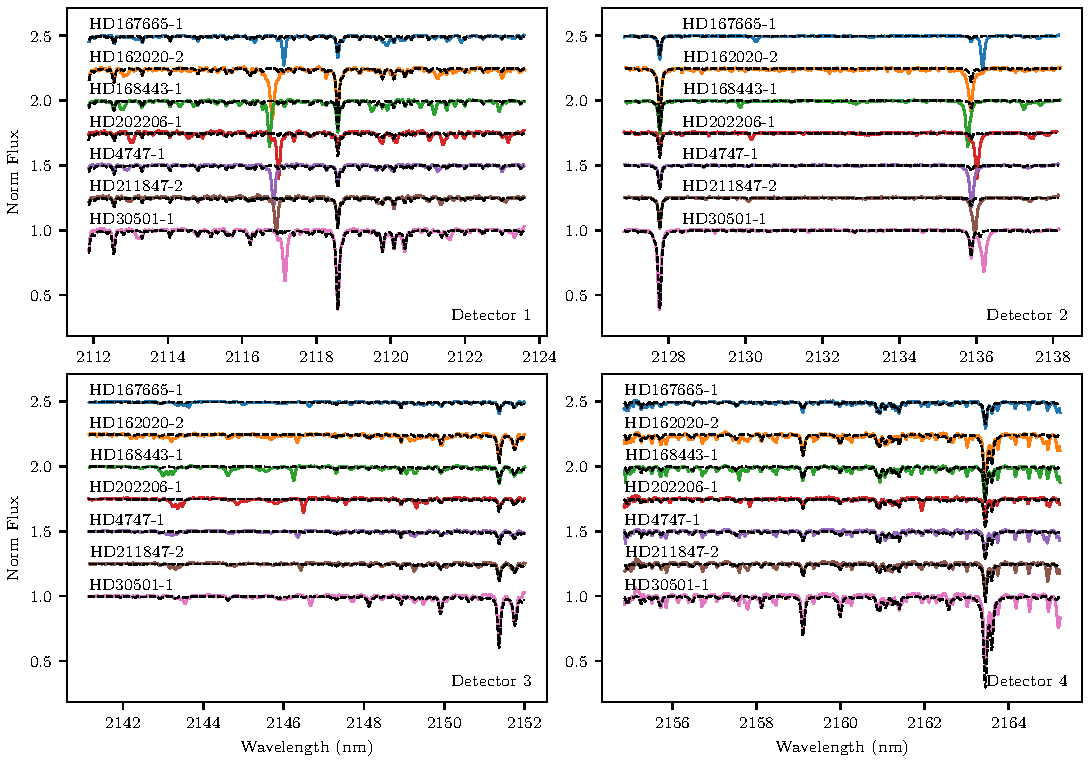
\includegraphics[width=1\linewidth]{figures/reduction/Spectra_examples}
    \caption[Example reduced CRIRES spectra for each target.]{An example spectra for each target and each detector \#1--4 in order of increasing wavelength.
       The solid lines are the spectra while the black dashed lines are the telluric models used for wavelength correction, showing good alignment with the spectra.}
    \label{fig:spectraexamples}
\end{figure}

In hindsight using the wavelength solution from the {ESO} pipeline may have been a good starting point, rather than the pixel positions, for calibration of the {DRACS} reduced spectra.
This may have made the line identification simpler.

In simulations of a differential technique similar to what is presented in \cref{cha:direct_recovery}, \citet{kostogryz_spectral_2013} simulate the affect of wavelength calibration errors on differential result.
They found that calibration error >0.1 pixels will produce signals greater than the photon noise level in spectra with a \snr{} of around 500.
They show that this upper limit only just the level achieved by~\citep{brogi_signature_2012} calibrated using the telluric lines from the observation.
This shows how important the wavelength calibration is to detect the spectra of the companion.


\subsection{Telluric correction}
\label{subsec:telluric_correction_application}
After wavelength calibration telluric correction is performed using the same {TAPAS} atmospheric transmission models.
When inspecting the models and observations there was slight difference in the airmass, $m$, between the synthetic spectra and the airmass in the fits header.
The depth of the telluric lines were re-scaled to match the airmass of the observations using the relation \(\rm T = T^{\beta}\), where \(\rm T\) is the transmission of the telluric spectrum and \(\beta\) is the airmass ratio between the observation and model $\beta ={m_{observed}/m_{model}}$.
This scaling adjusted the depth of most absorption lines to better match the observations, but does not correctly scale the deeper \ce{H2O} lines, for which there were still differences.

The scaled telluric model is interpolated to the wavelengths of the observed spectrum and then used to correct the observed spectra through division, leaving behind a telluric corrected spectra.
Telluric spectra used for correction can be observed alongside the non-corrected spectra in \cref{fig:spectraexamples} as the black dashed lines.

\subsubsection{Separate \ce{H2O} scaling.}
A technique suggested by~\citet{bertaux_tapas_2014} was attempted to address the poor \ce{H2O} airmass scaling.
This involved fitting a scaling factor to the \ce{H2O} absorption lines before convolution to the instrument resolution.
This was achieved by first dividing the spectrum by a telluric model containing the non-\ce{H2O} constituents, convolved to the observed resolution, and scaled by the airmass to remove the non-\ce{H2O} lines.
Then the telluric model with only \ce{H2O} lines at full resolution was scaled by a factor \(\textrm{T}^{x}\) and convolved to the instrumental resolution\footnote{\(\rm R=50\,000\) for this work} and compared to the remaining telluric lines in the observed spectra.
This scaled and convolved model was fitted to the observations to find the best was fitted to find the best scaling factor \(x\), for the \ce{H2O} lines.

It was found that for a few spectra in the sample this method corrected the deeper telluric lines well, but in many cases the fitted scaling factor was affected by the presence of blended stellar lines (attempting to fit those also).
It was also strongly influenced by the deepest \ce{H2O} telluric lines present.
The telluric correction of the deep \ce{H2O} lines could be improved with this technique, but at the cost of worsening the correction of the many smaller \ce{H2O} lines.
Since the smaller \ce{H2O} lines covered more of the spectrum in this region than the larger lines, the separate \ce{H2O} scaling was not continued.
One possible solution for this would be to perform a piece-wise telluric correction, performing this step only for the deeper \ce{H2O} lines.
This technique could also benefit from a larger wavelength span that would enable blended lines to be ignored while having sufficient deep \ce{H2O} lines to fit the scaling factor correctly.
This small experiment shows that a simple scaling is not enough to correct for the absorption of \ce{H2O} in an effective way, for this case.
Another better solution would be using proper atmospheric fitting tools that fits the telluric model to the observations, such as {Molecfit}, in which the atmospheric composition can be changed to match the observed telluric line strengths.


\subsection{Wavelength masking}
Throughout the course of this work several wavelength regions were found where the extraction could not be performed reliably due to the wavelength calibration and telluric line corrections.
Different wavelength masks are applied to these areas to remove them from the spectra.
The main reasons that wavelength masking is used are collated below.

Firstly, regions near the edges of each detector where the wavelength solution is extrapolated outside of the calibrating telluric lines are removed, reducing the effective size of each detector by about \(10\%\) or \(\sim\)100 pixels.

Secondly, any remaining artefacts present in the spectra and the centres of deep telluric lines where telluric correction was not corrected properly are masked out.
The telluric correction sometimes results in ``emission-like'' peaks in the corrected spectrum, which are removed.
These factors combined result in masking out around a further 10\% of the observed spectra.

In \cref{sec:chi2_results} a further wavelength restriction is applied to mask out regions where there is a large mismatch between the observed spectrum and the closest synthetic spectra to the host.
This significantly restricts the wavelength span utilized for that purpose to around only 43\%.
The masked regions created by this last mask are shown in \cref{fig:visualinspection-hd2118471}.


\subsection{Barycentric {RV} correction}
\label{subsec:barycentriccorrection}
After the telluric correction is performed, the spectra are corrected for Earth's barycentric motion.
The orbital and rotational motion of the Earth imparts a daily and seasonal radial velocity measurement offset onto observations.
To accurately compare the radial velocity (or spectral shift) between two measurements, they need to be translated into a common rest frame.
The rest frame of choice is the barycentre of the Solar System.
Equations to relate the observed spectral shift to the {RV} shift at the \textit{Barycentric Celestial Reference Reference System}~\citep{rickman_transactions_2001} rest frame are provided in~\citet{lindegren_fundamental_2003}.

In this work the barycentric velocity correction is calculated using PyAstronomy's\footnote{https://pyastronomy.readthedocs.io} \emph{helcor} function ported from the REDUCE IDL package (see~\citet[][]{piskunov_new_2002}).
This calculates radial velocity of the observer towards the astronomical target, accounting for Earth's barycentric motion as well as Earth's rotation.
This computation requires the date and time of the observation, the location of the observatory and the celestial coordinates of the target.
The observed spectra are Doppler shifted by the negative value of the barycentric velocity calculated, placing all spectra as if they were observed from the barycentre of the Solar System.

The maximum barycentric velocity of the Earth is around 30\kmps{}.
It is common to see spectral regions $\pm30$\kmps{} either side of telluric lines with an absorption depth >2\% avoided in analysis (such as {RV} determination), as these will be affected by the telluric lines at some point in the year.

